\chapter{Comparison of Existing Recommender Systems}

The recommendations used for this trial were 

\begin{itemize}
\item{$k$-Nearest Neighbor}
\item{Support Vector Machines}
\item{Matchbox: Matchbox MF  + L2 Regularization}
\item{Social Matchbox: Matchbox MF + Social Regularization + L2 Regularization}
\end{itemize}

Social Matchbox uses the Social Regularizer to incorporate the social aspect of the data, while SVM incorporates the social information in the $\f_{\x,\z}$ features it uses. Matchbox and Nearest Neighbors do not make use of any social information and are collaborative filtering recommenders.

\section{Online Results}

The first live user trial was run from August 1 to October 13. The algorithms were randomly distributed among the 106 users who installed the LinkR application. Each user was recommended 3 links everyday and they were able to rate the links on whether they 'Liked' or 'Disliked' it. 

Social Matchbox and Support Vector Machines, the two algorithms that make use social information, garnered the most number of likes from the LinkR users, with Social Matchbox edging out SVM by just 4 likes. This suggests that using social information does indeed provide useful information that results in better recommendations.

When it comes to the number of dislikes, SVM garnered the most number of dislikes by a big margin. Social Matchbox and Matchbox came next, with Nearest neighbors having the least number of both likes and dislikes. Because Social Matchbox received the highest ratio of likes to dislikes among all the four algorithms, we considered Social Matchbox to be the best performing recommendation algorithm in this first trial.

\begin{table}[h!]
\centering
\begin{tabular}{| l | c |}
\hline
{\bf Algorithm} & {\bf Users} \\
\hline
Social Matchbox & 26\\
Matchbox  & 26 \\
SVM & 28 \\
Nearest Neighbor & 28 \\
\hline
\end{tabular}
\caption{Number of Users Assigned per Algorithm.}
\end{table}

\begin{figure}[h!]
\centering
\subfigure{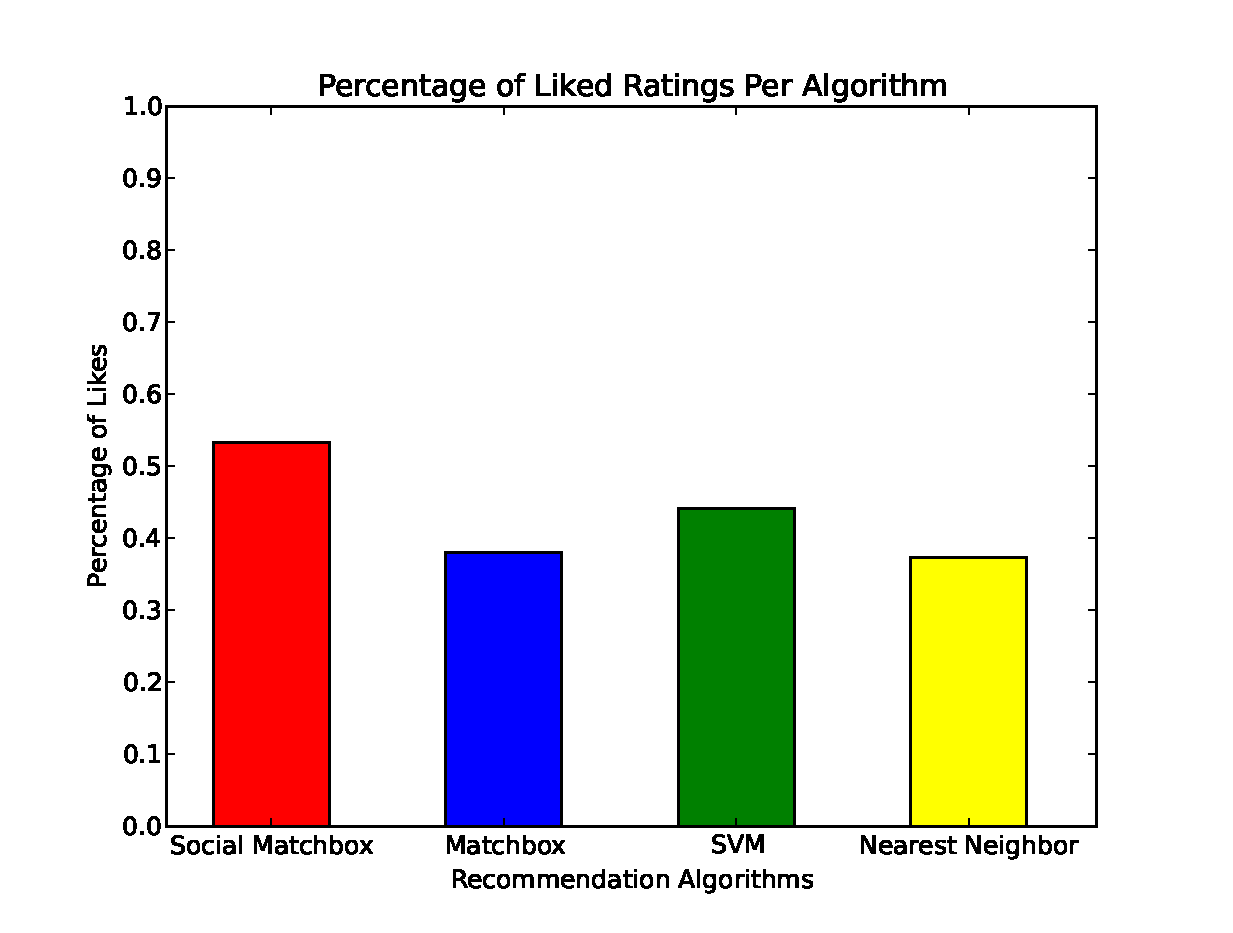
\includegraphics[scale=0.35]{img/live-likes1.eps}}
\subfigure{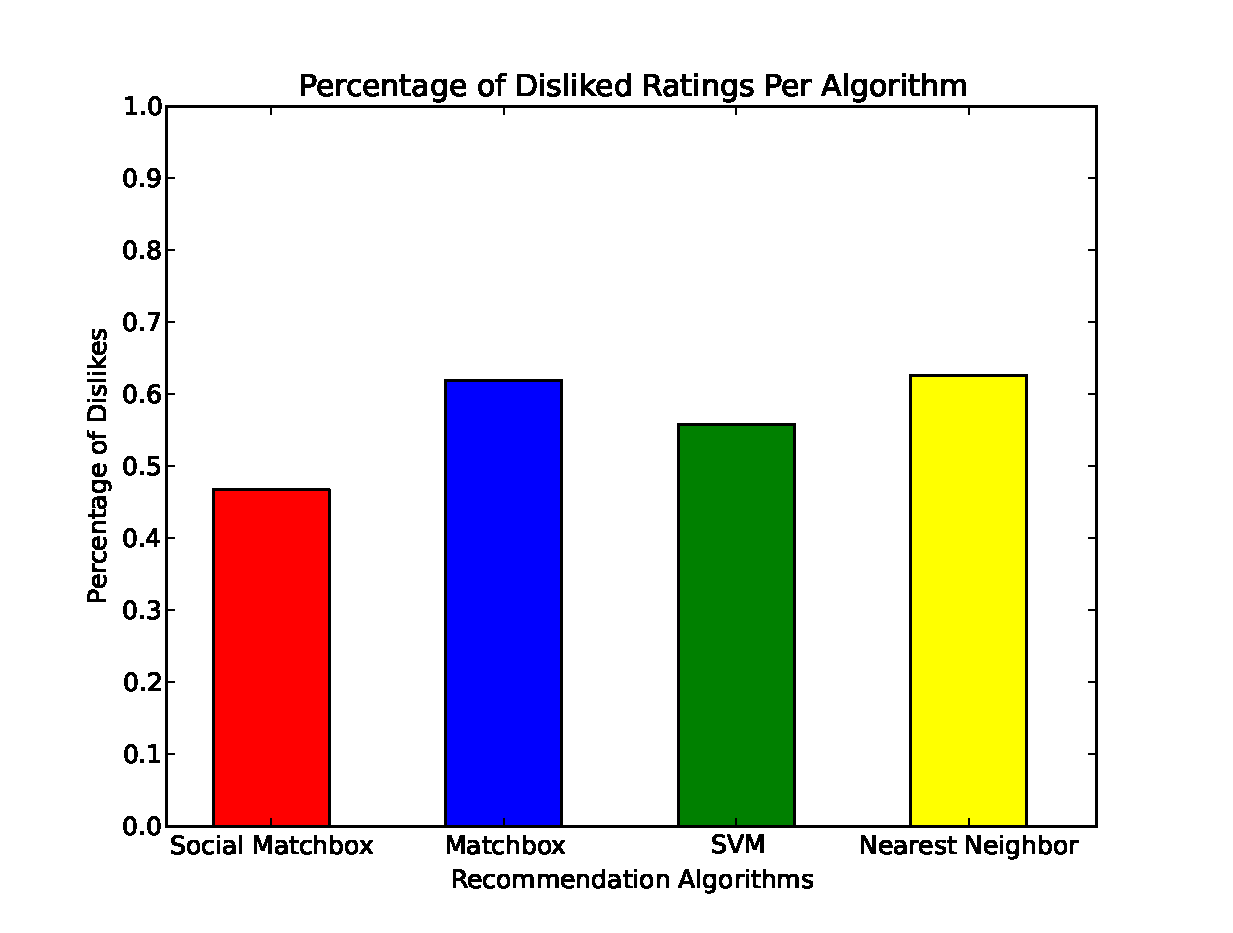
\includegraphics[scale=0.35]{img/live-dislikes1.eps}}
\caption{Results of online live trials}
\end{figure}

\section {Passive Results}

The goal of the passive experiments was to see how best to reproduce the results of the live experiments offline. We tried out the different splitting combinations of training and testing data detailed in the last chapter, and found that training on the UNION dataset and and testing on the APP-USER-ACTIVE-ALL dataset best reflected the results of the online trials.

Additionally, the offline testing was used to tune the $\lambda$ parameters for the different algorithms.

\begin{figure}[h]
\centering
\subfigure{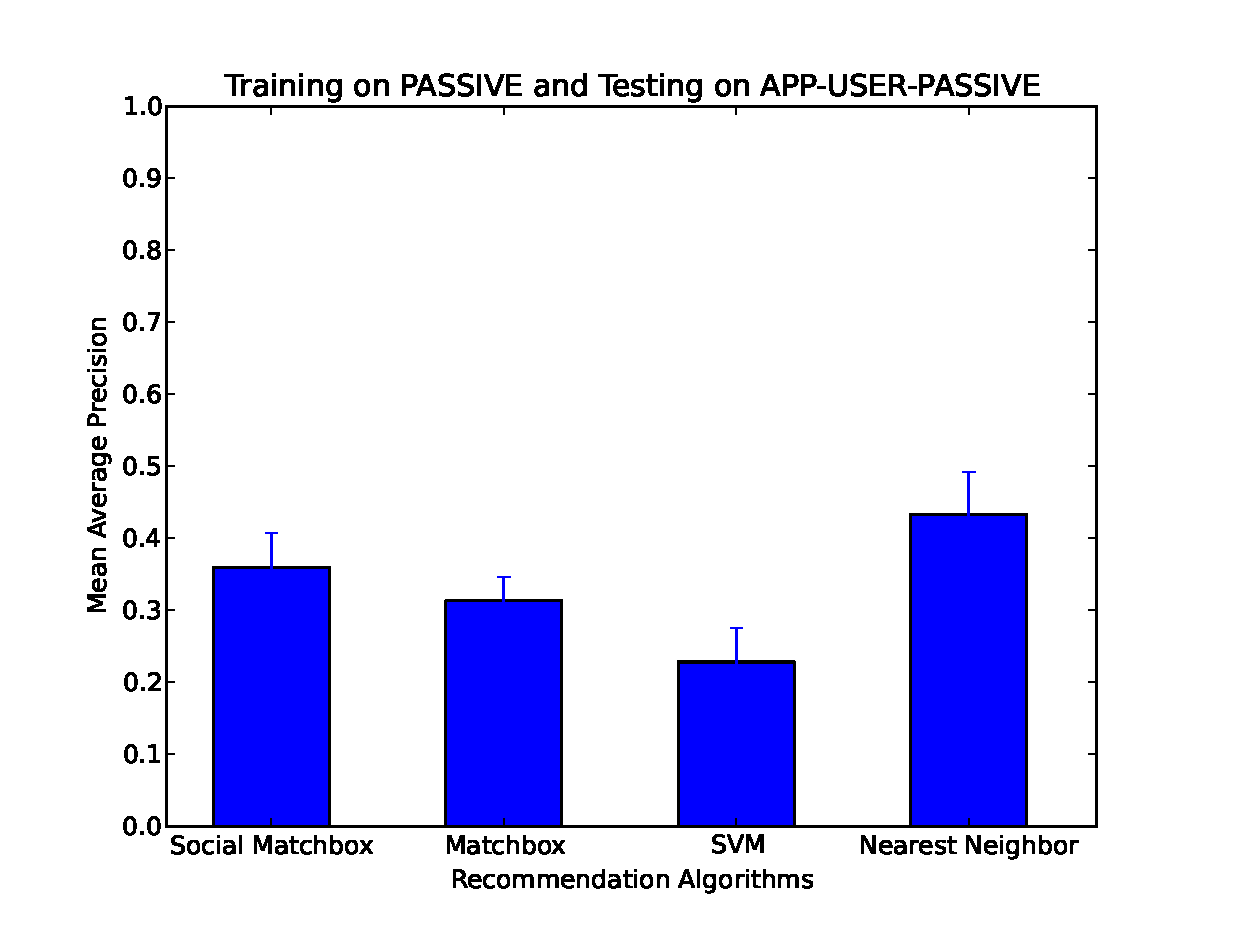
\includegraphics[scale=0.35]{img/Passive_App-User-Passive1.eps}}
\subfigure{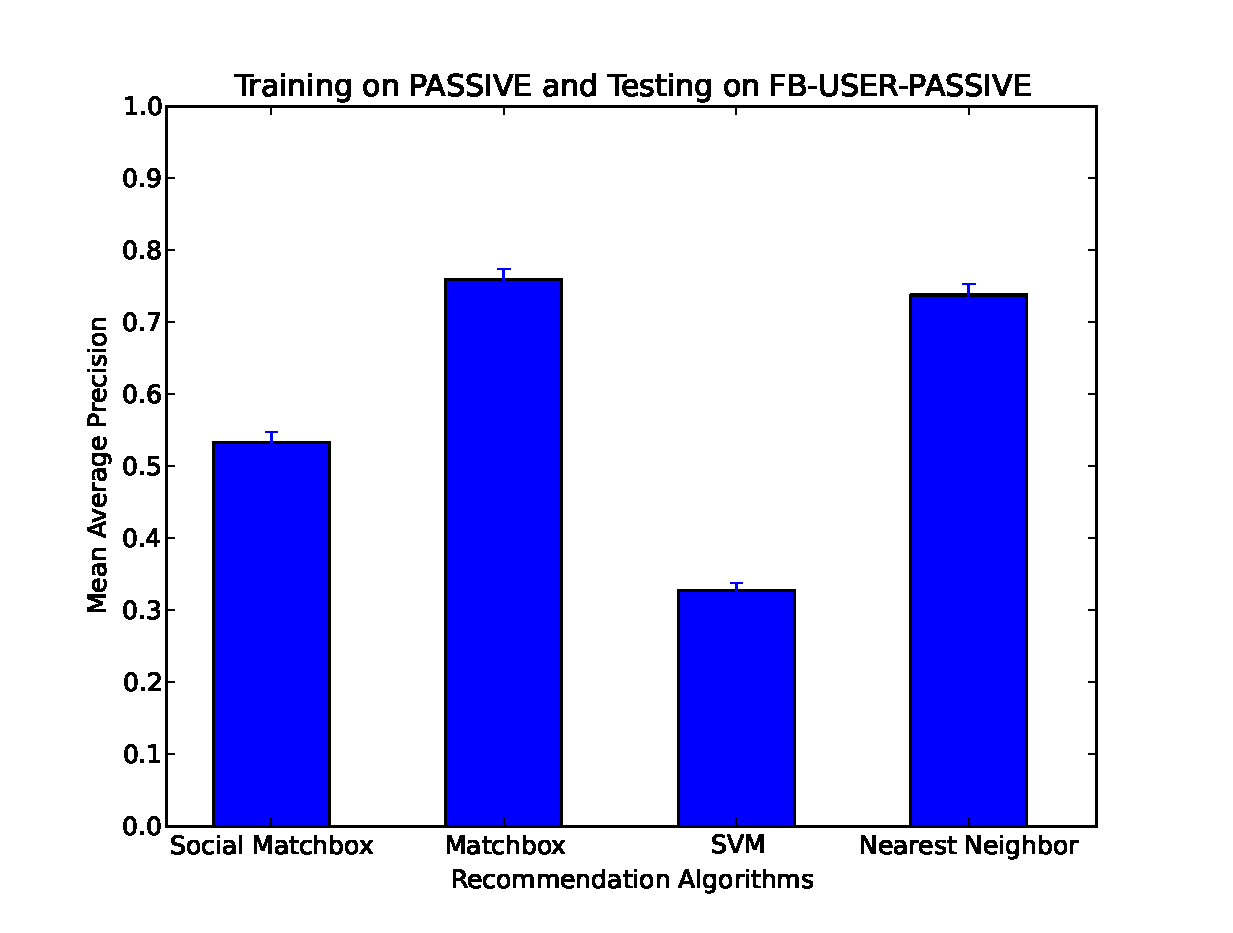
\includegraphics[scale=0.35]{img/Passive_FB-User-Passive1.eps}}
\subfigure{\includegraphics[scale=0.35]{img/Passive_App-User-active-all1.eps}}
\subfigure{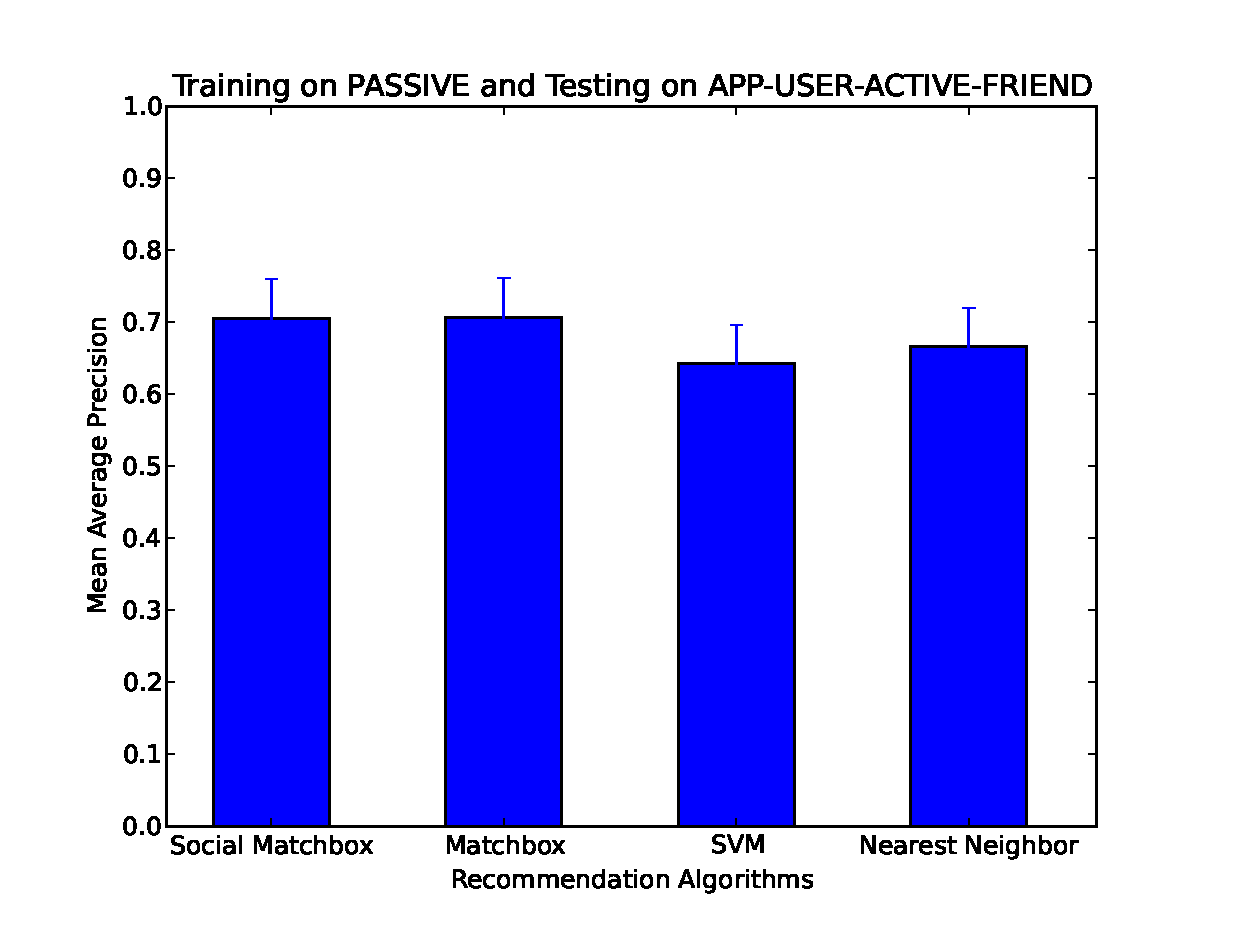
\includegraphics[scale=0.35]{img/Passive_App-User-Active-Friends1.eps}}
\subfigure{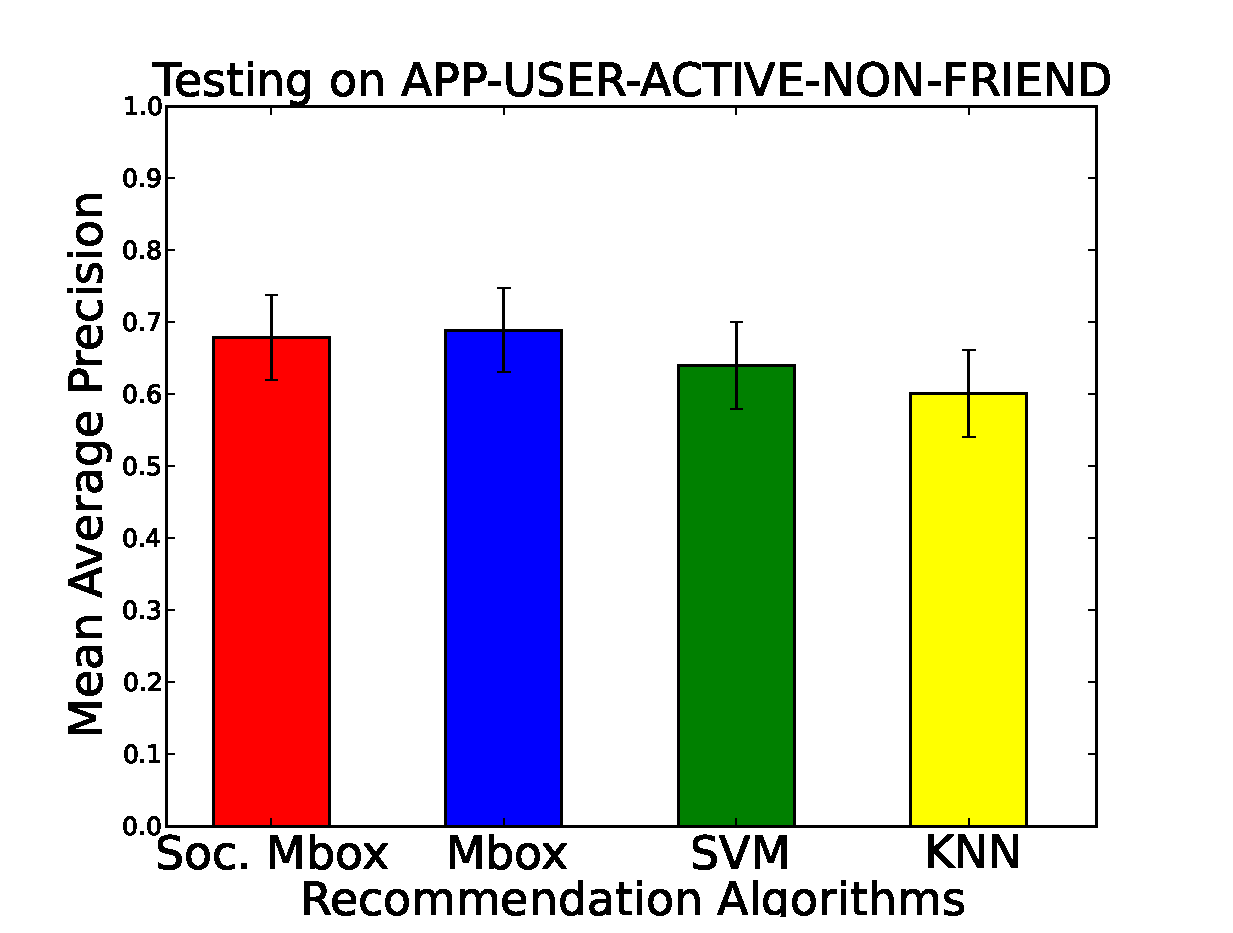
\includegraphics[scale=0.35]{img/Passive_App-User-Active-NonFriends1.eps}}
\caption{Results of training on Passive data}
\end{figure}

\begin{figure}[h]
\centering
\subfigure{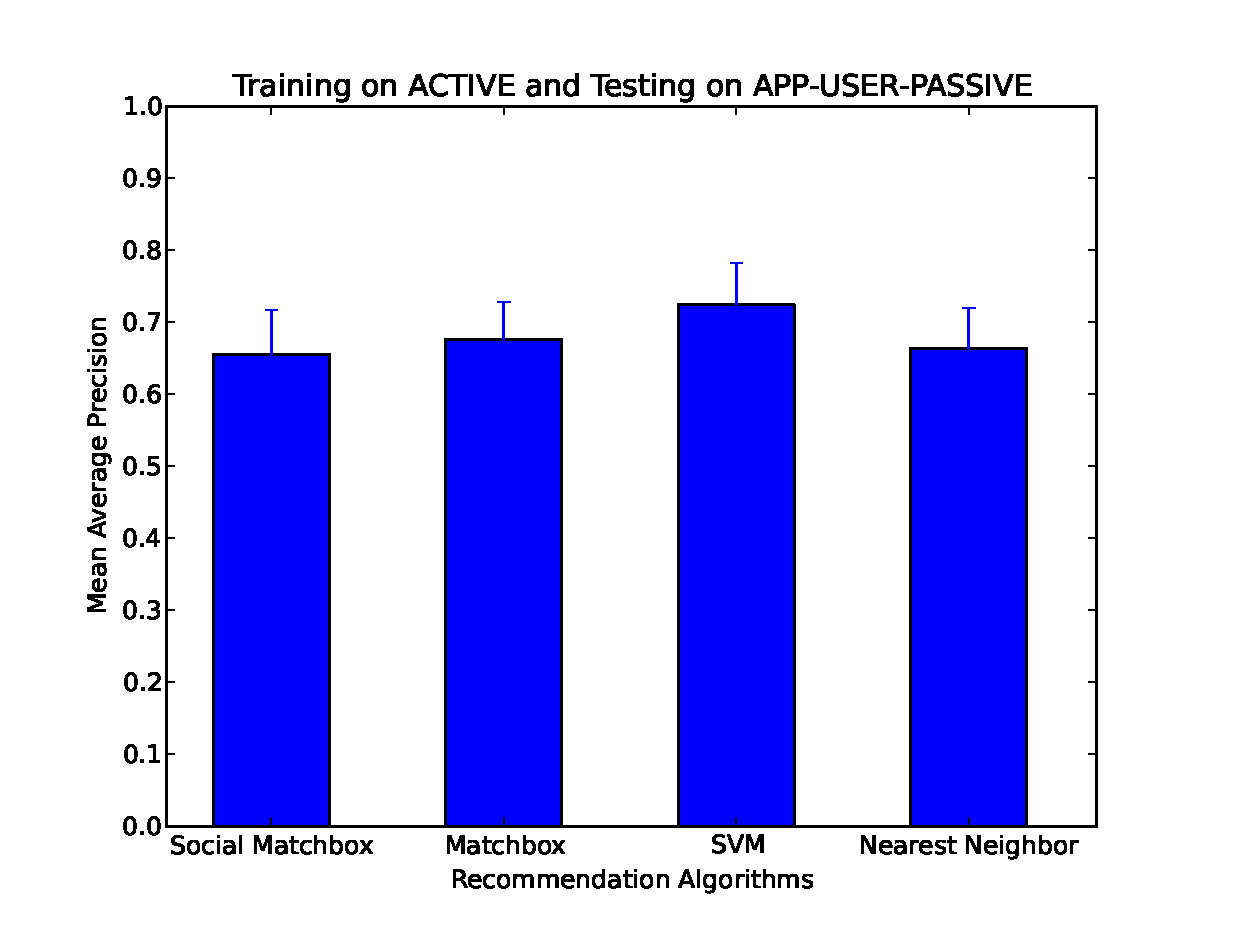
\includegraphics[scale=0.35]{img/Active_App-User-Passive1.eps}}
\subfigure{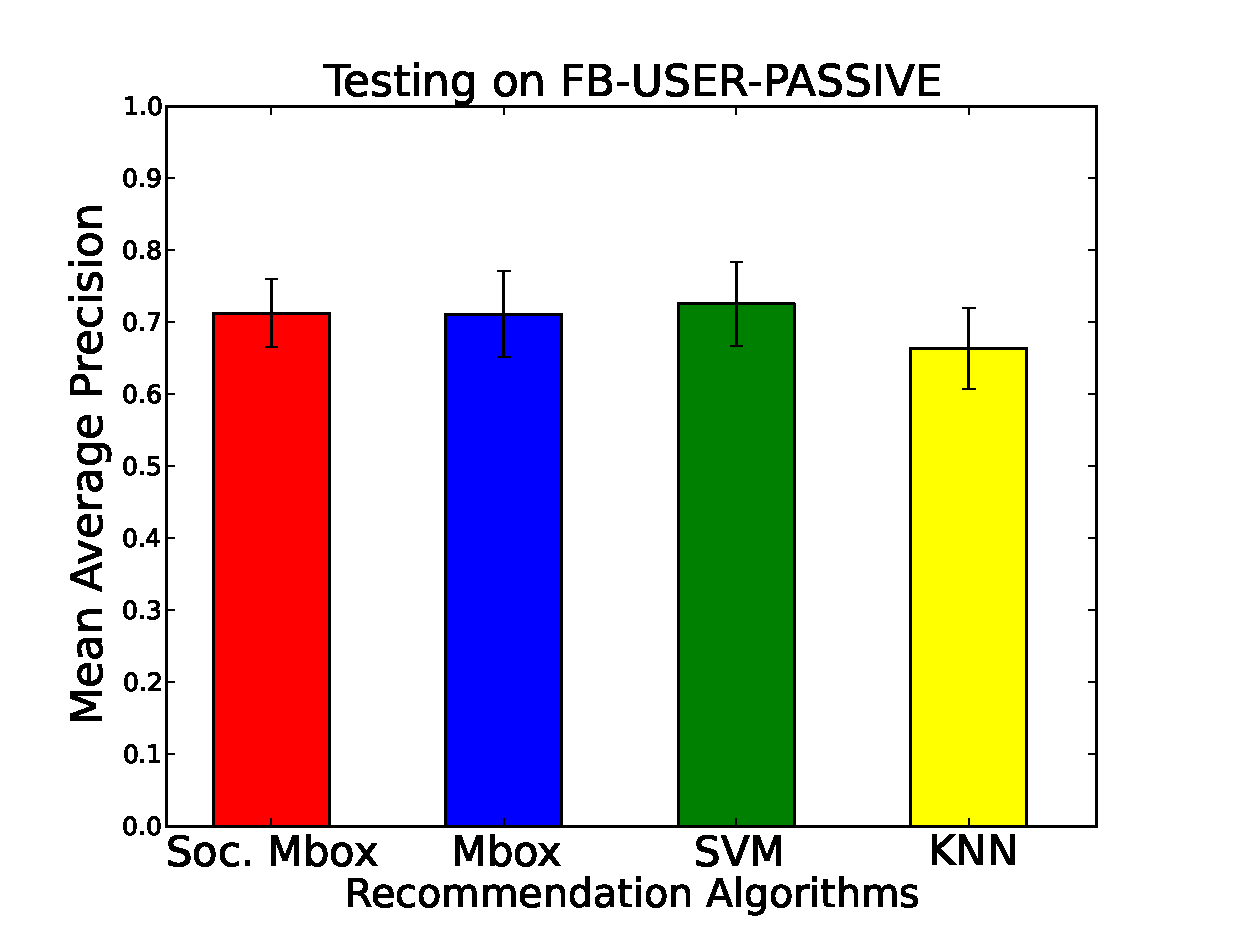
\includegraphics[scale=0.35]{img/Active_FB-User-Passive1.eps}}
\subfigure{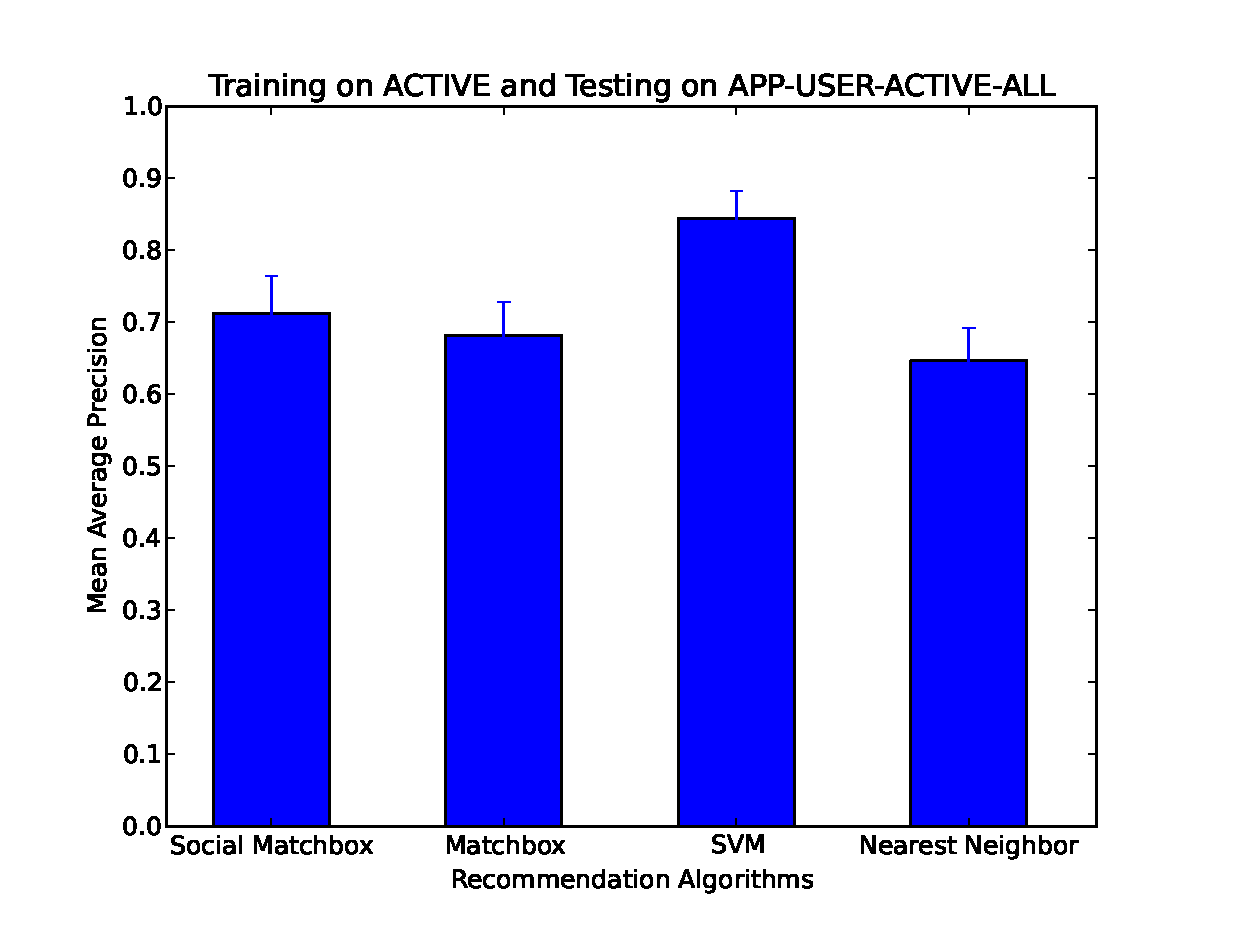
\includegraphics[scale=0.35]{img/Active_App-User-Active-All1.eps}}
\subfigure{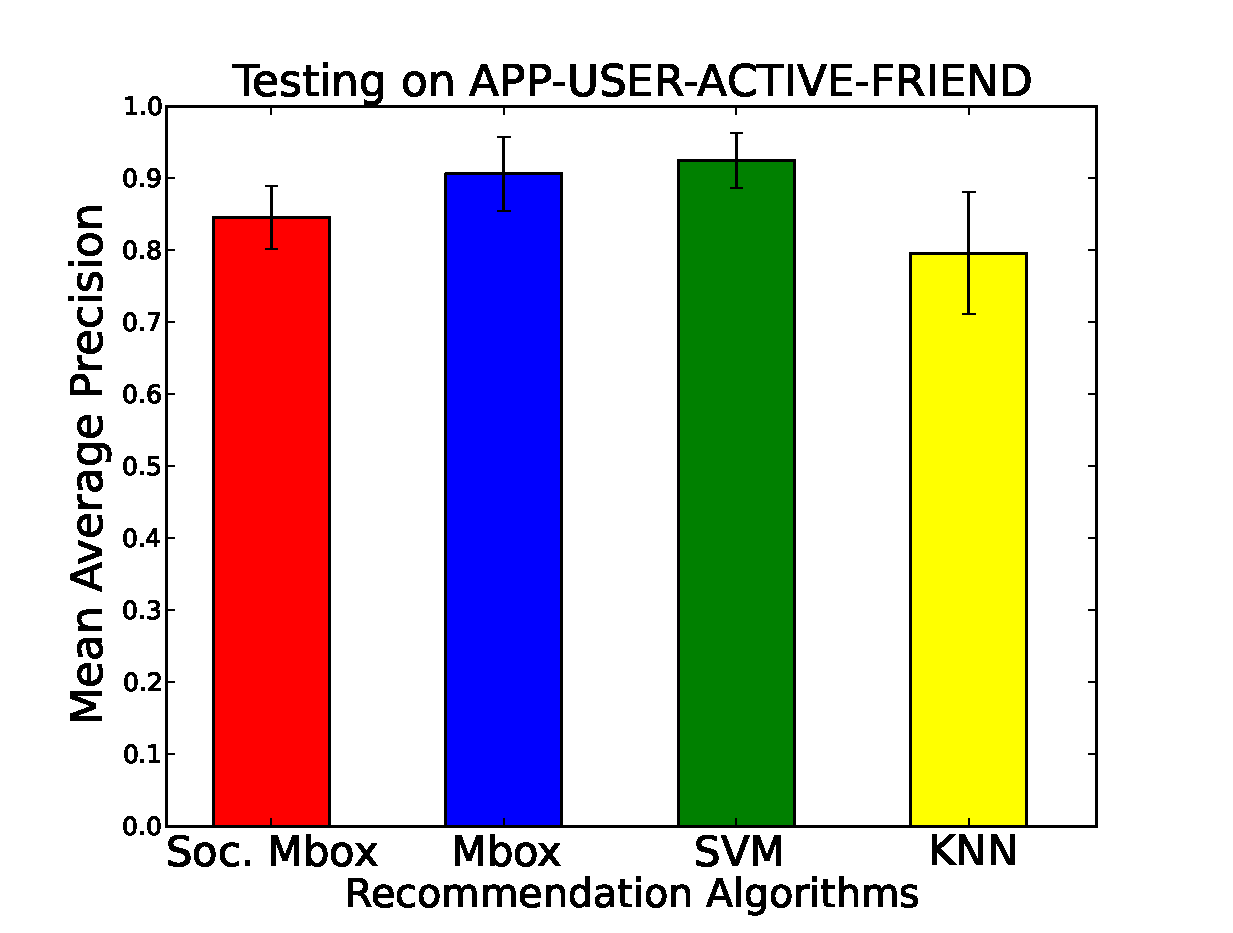
\includegraphics[scale=0.35]{img/Active_App-User-Active-Friends1.eps}}
\subfigure{\includegraphics[scale=0.35]{img/Active_App-User-Active-Nonfriends1.eps}}
\caption{Results of training on Active data}
\end{figure}

\begin{figure}[h]
\centering
\subfigure{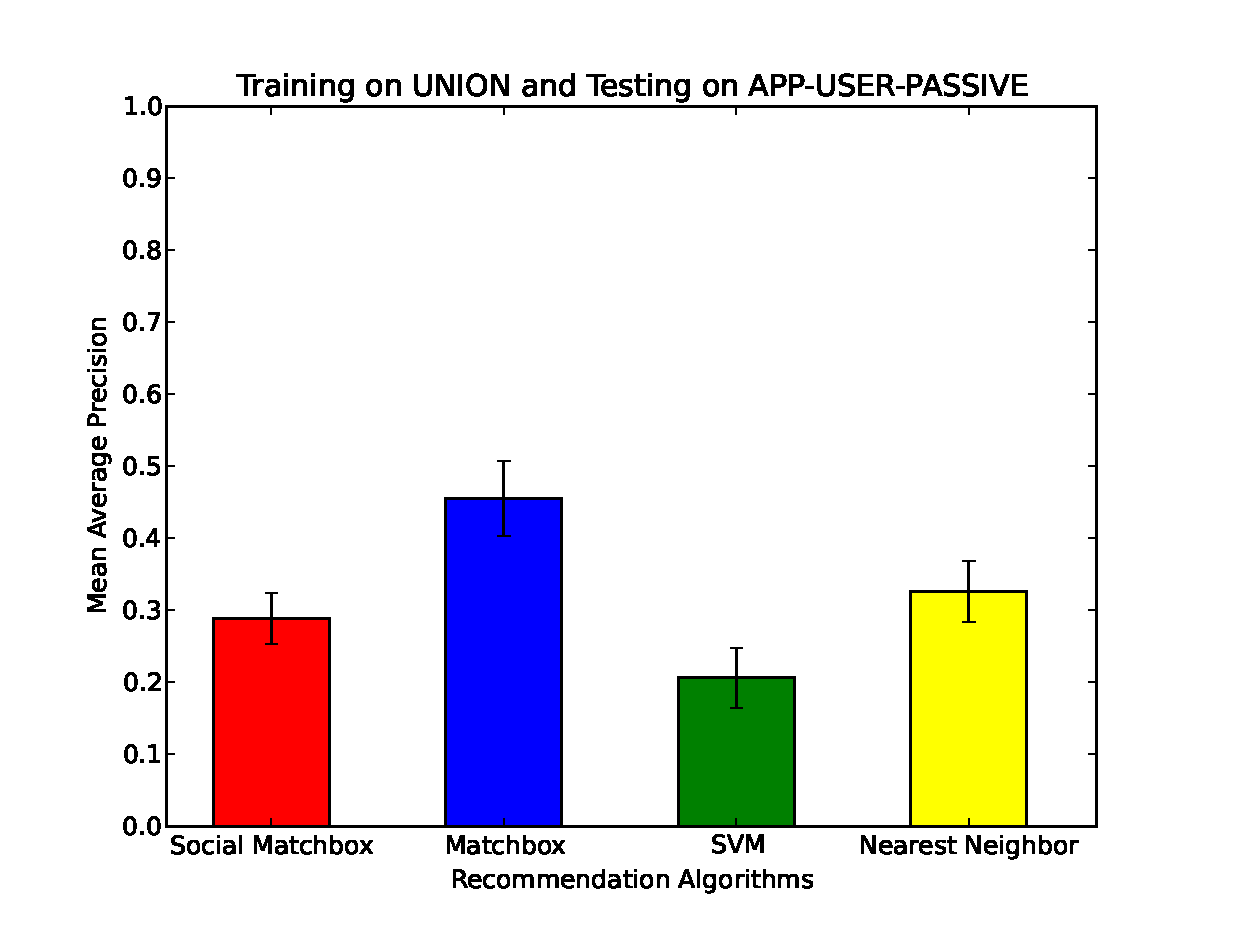
\includegraphics[scale=0.35]{img/Union_App-User-Passive1.eps}}
\subfigure{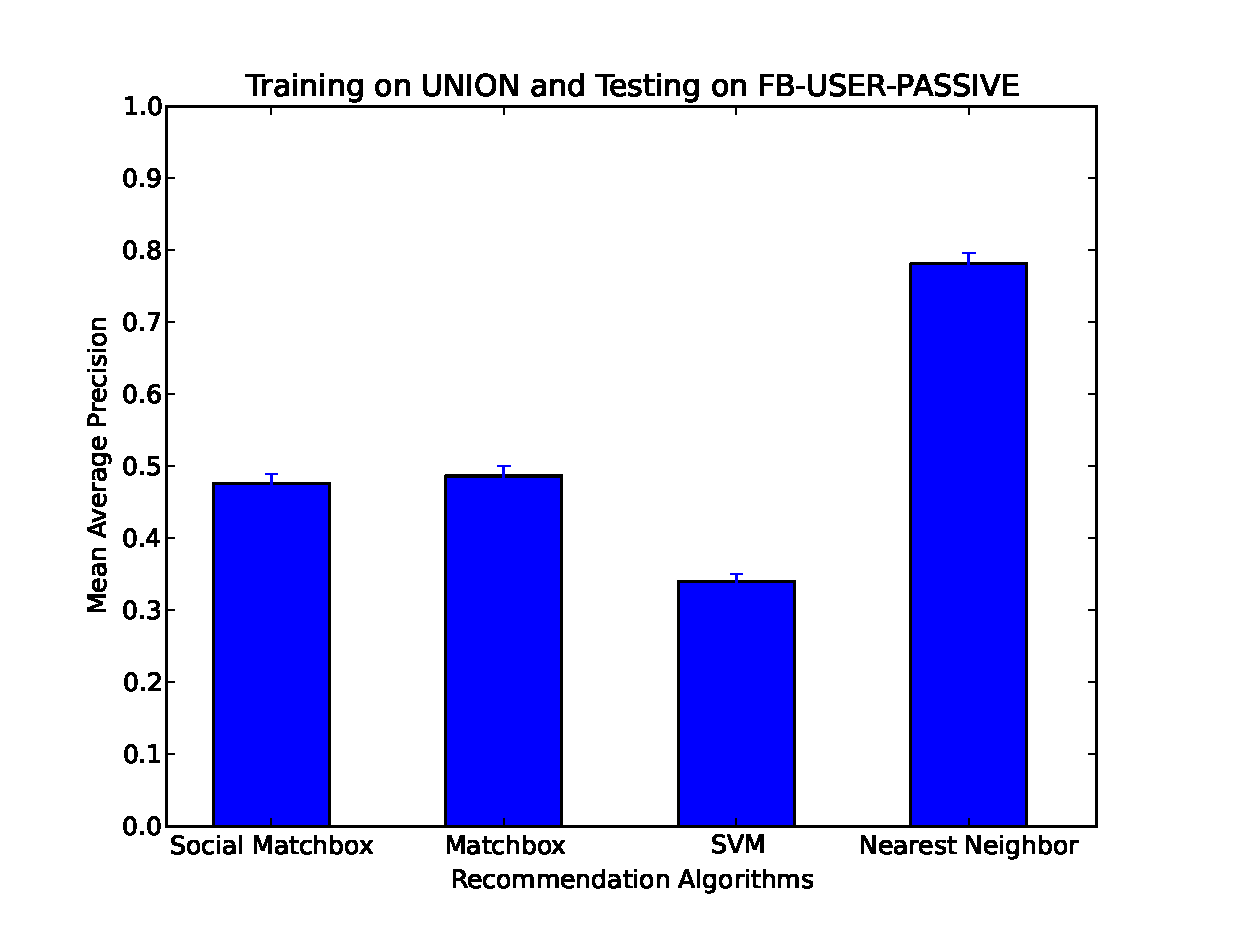
\includegraphics[scale=0.35]{img/Union_FB-User-Passive1.eps}}
\subfigure{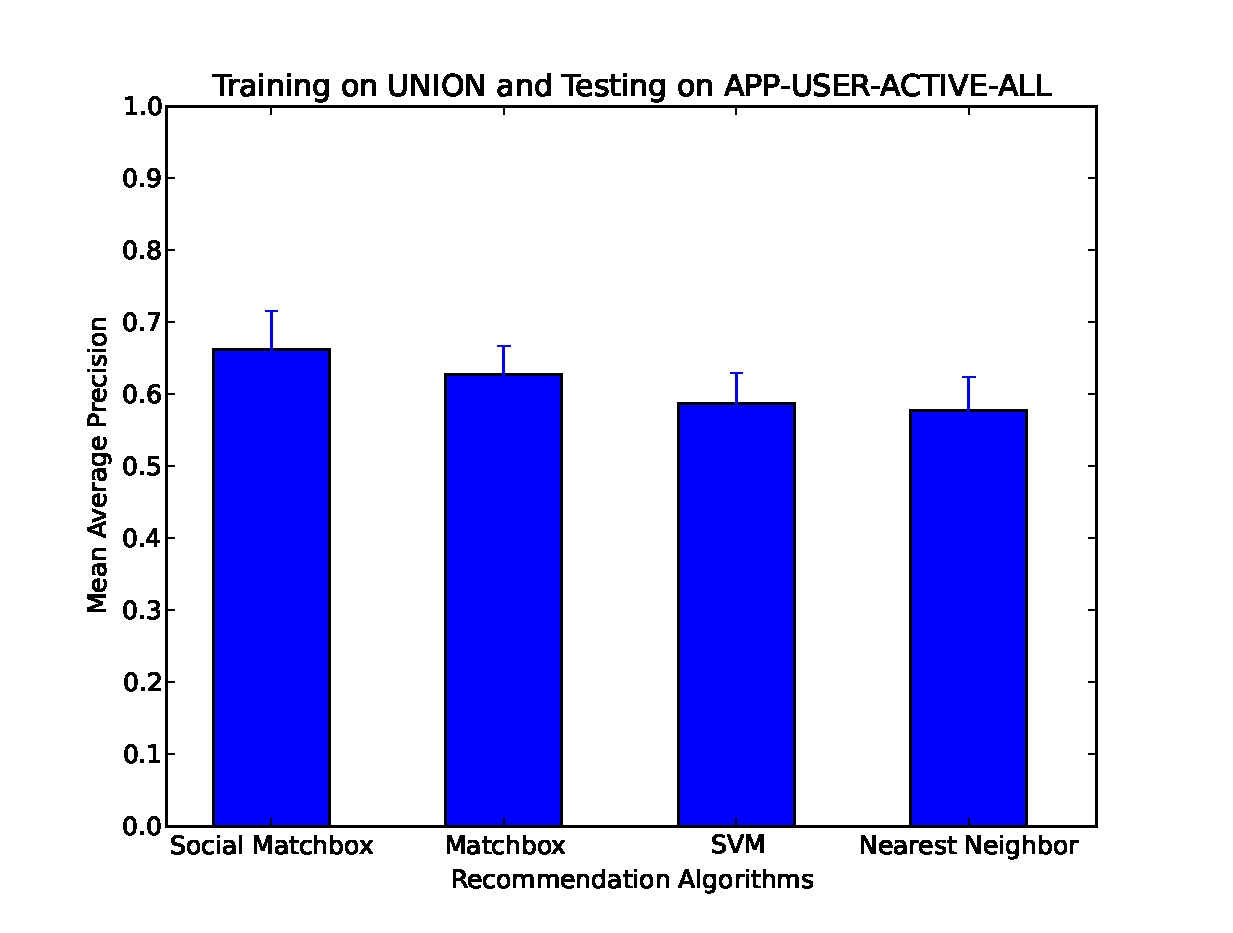
\includegraphics[scale=0.35]{img/Union_App-User-Active-All1.eps}}
\subfigure{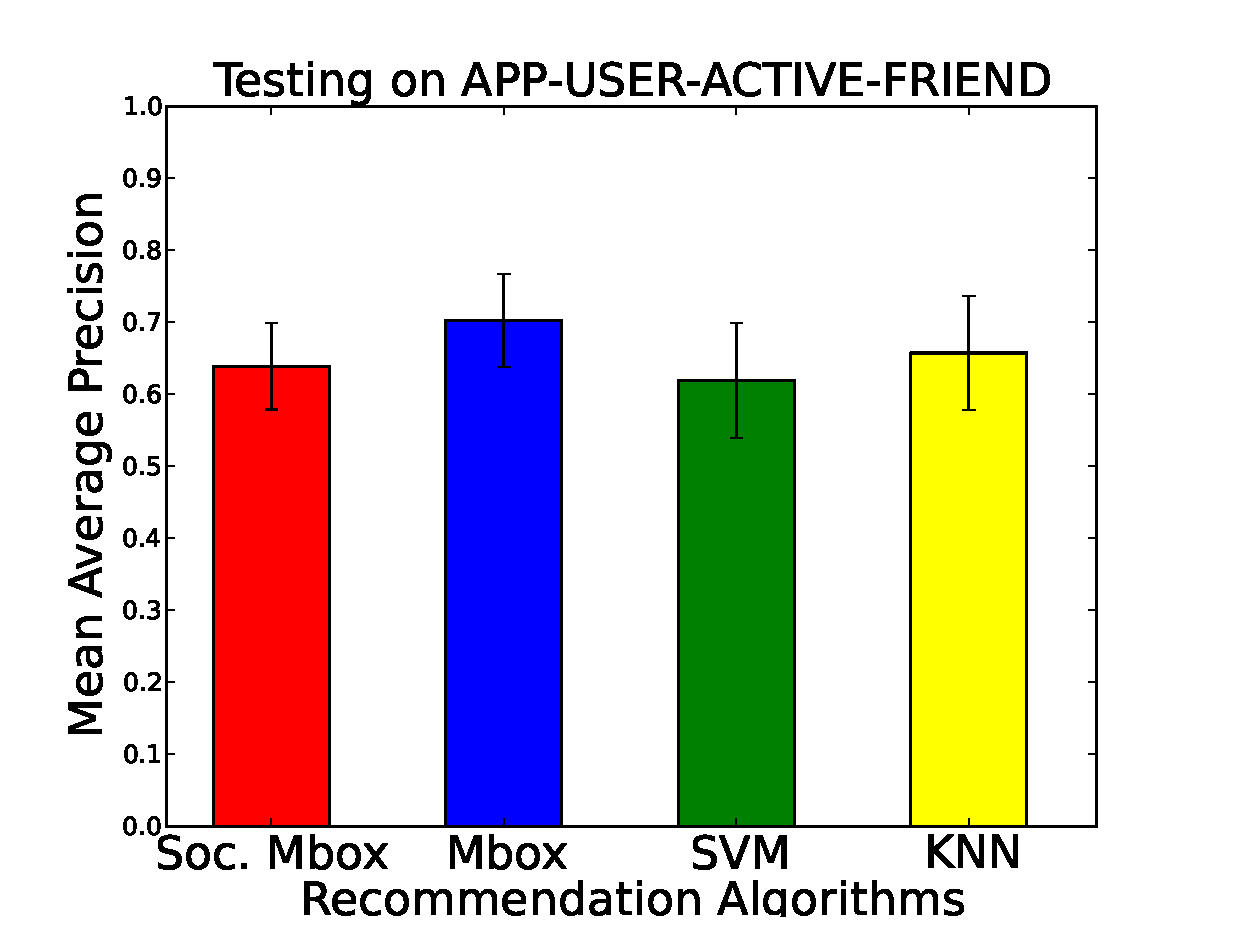
\includegraphics[scale=0.35]{img/Union_App-User-Active-Friends1.eps}}
\subfigure{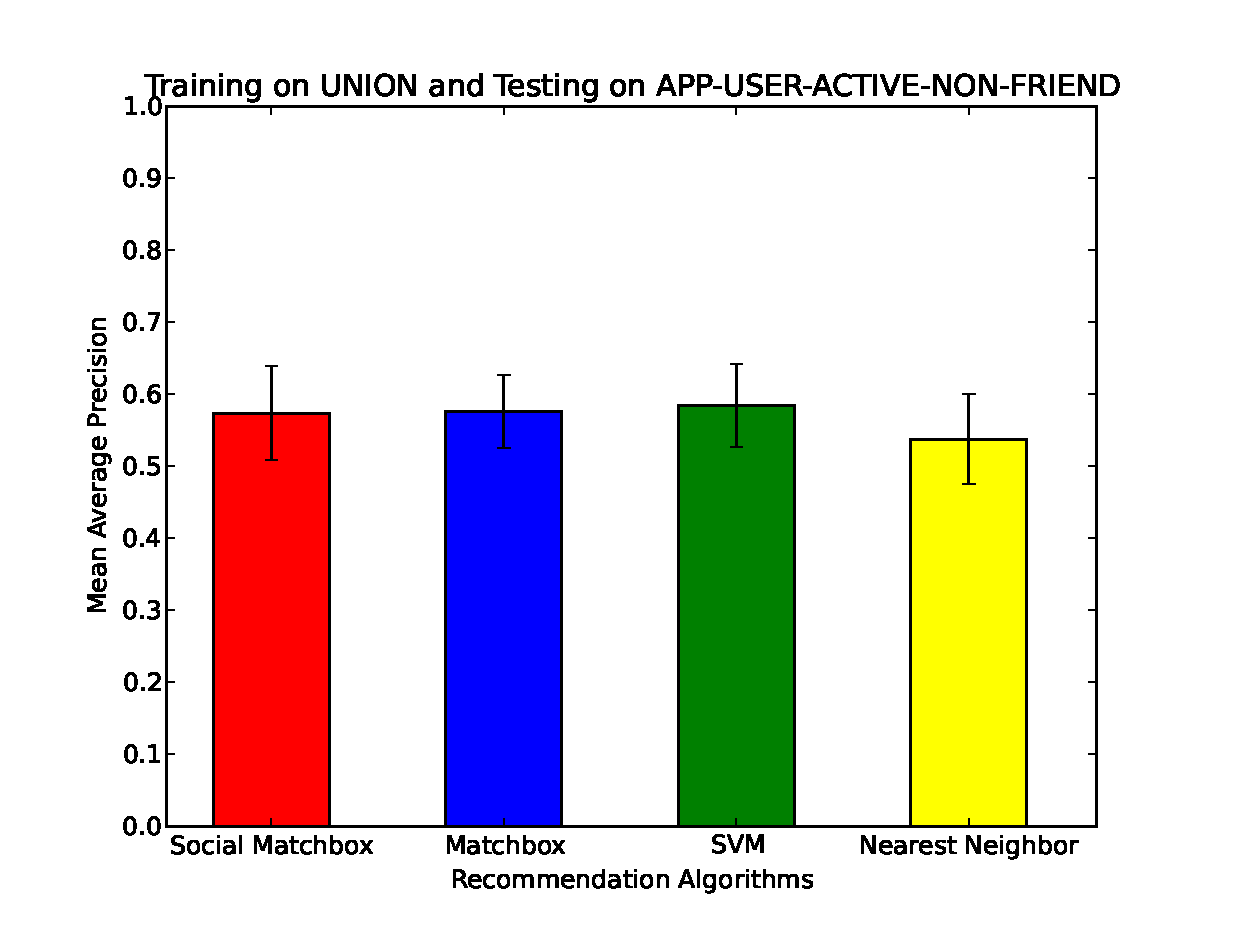
\includegraphics[scale=0.35]{img/Union_App-User-Active-NonFriends1.eps}}
\caption{Results of training on Union data}
\end{figure}

\section{Survey Results}

Near the end of the first trial, the LinkR users were invited to answer a survey regarding their experiences with the recommendations they were getting. They were asked a number of questions, with the following pertaining to the quality of the recommendations:

\begin{itemize}
\item{Do you find that ANU LinkR recommends interesting links that you may not have otherwise seen?}
\item{Do you feel that ANU LinkR has adapted to your preferences since you first started using it?}
\item{How relevant are the daily recommended links?}
\item{Overall, how satisfied are you with LinkR?}
\end{itemize}

They gave their answers to each question as an integer rating with range $[1-5]$, with a higher value being better. Their answers were grouped together according to the recommendation algorithm that was assigned to them, and the averages per algorithm are below.

One more, we see that Social Matchbox achieved higher scores than the other recommendation algorithms, in all four questions. The results of the survey reflected the results in the online live trial and confirms that Social Matchbox was the best recommendation algorithm in the first trial.
 
\begin{figure}[h]
\centering
\subfigure{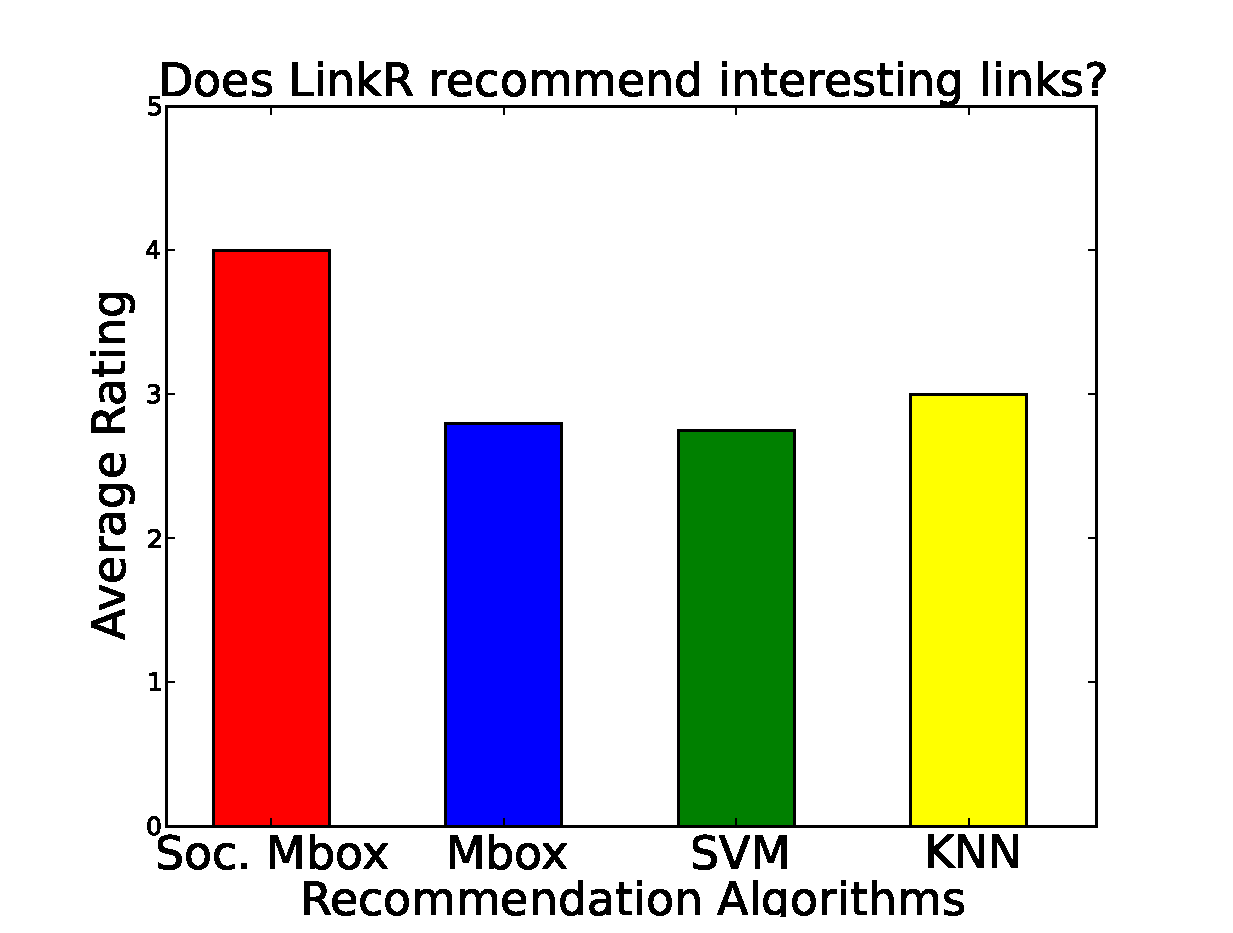
\includegraphics[scale=0.35]{img/not-seen.eps}}
\subfigure{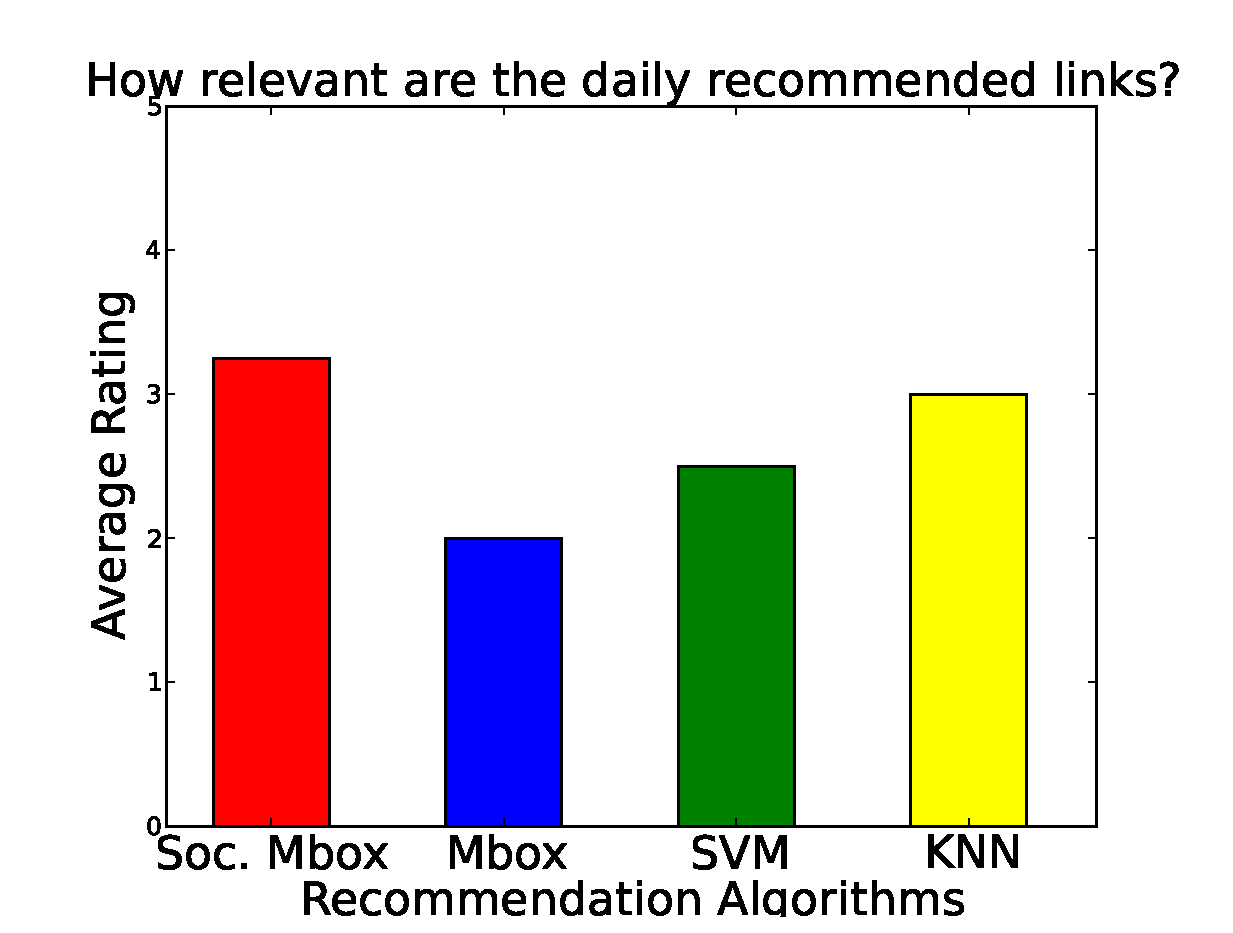
\includegraphics[scale=0.35]{img/relevant.eps}}
\subfigure{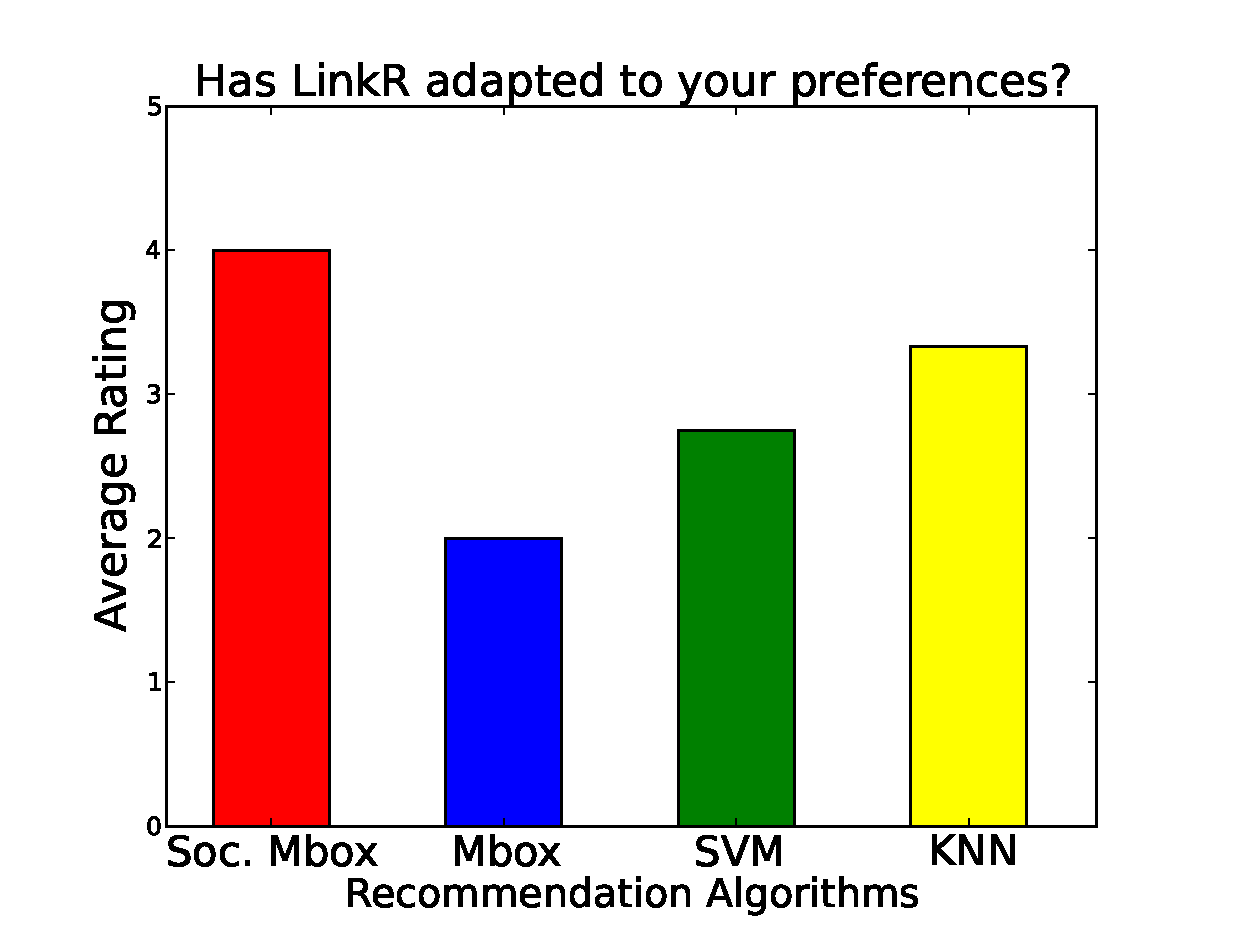
\includegraphics[scale=0.35]{img/adapted.eps}}
\subfigure{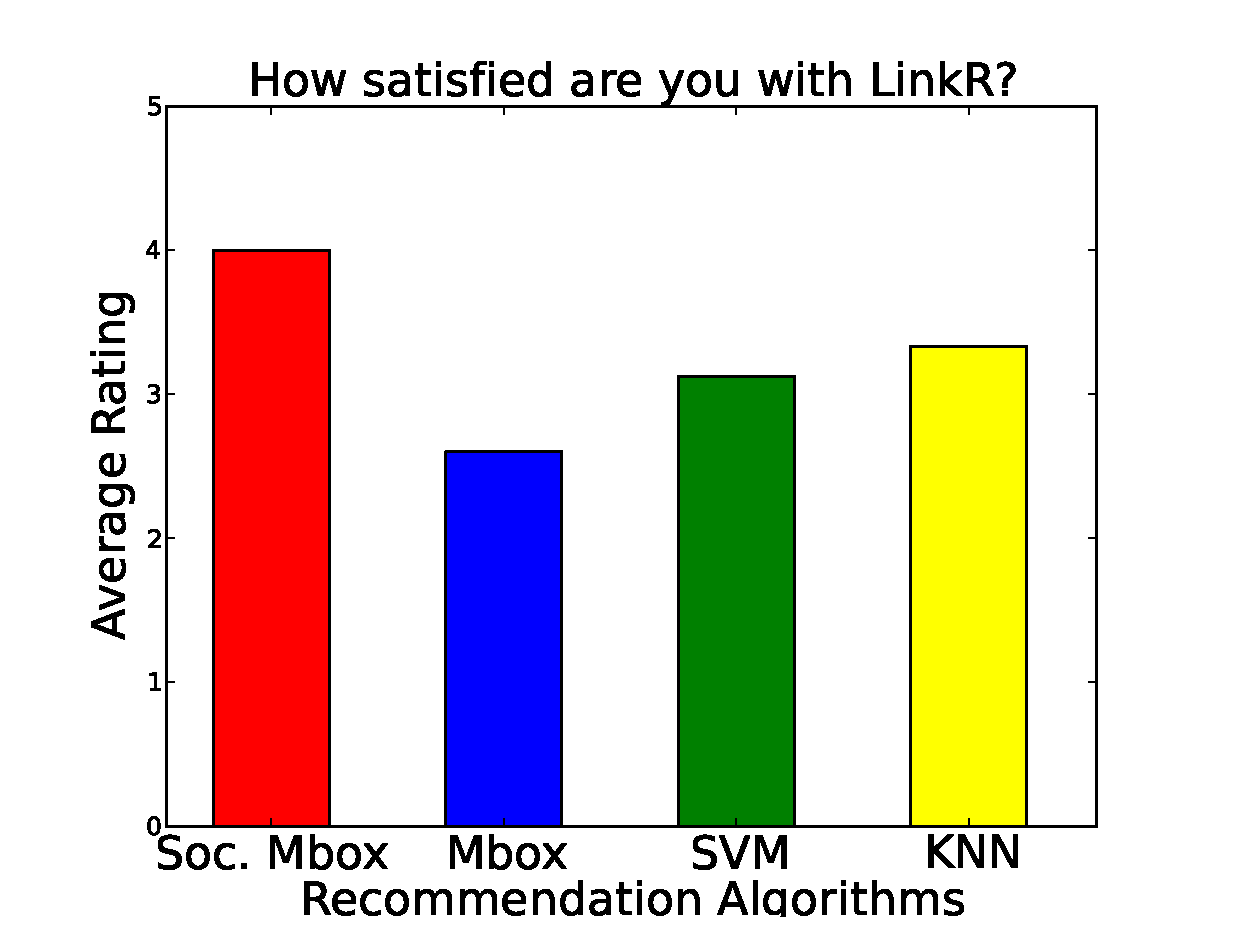
\includegraphics[scale=0.35]{img/satisfied.eps}}
\caption{Results of user survey after the first trial}
\end{figure}

